% Drawing 154/08-7 -- folder 154, batch 08, archive page 151 (PDF page 152).
% Transcription: page de dessins à l'encre et au crayon, sans texte : une vingtaine de disques traversés de pseudo-droites (brunes, noires, vertes), certains arcs du bord renforcés en vert ; dans plusieurs disques, les régions sont marquées alternativement de deux signes, l'un en forme de $\varepsilon$, l'autre en forme de chiffre $3$ à longue queue (un coloriage en deux classes, semble-t-il) ; dans un disque, une étoile de trois droites jaunes et noires, deux d'entre elles hachurées, un triangle central hachuré ; un disque divisé en secteurs par huit rayons ; des pentagones ; de petits disques verts ; deux longues droites au crayon traversent la page en croix
% Kind: about twenty disks with arrangements, regions marked with two alternating signs. Method 2 (schematic redraw from the facsimile). Status: partial.
% Notes: Page of ink and pencil drawings without text, over a job banner and job log (19 Aug 82; not reproduced): about twenty disks crossed by pseudolines (brown, black, green), some arcs of the rim reinforced in green; in several disks the regions are marked alternately with two signs (read as « epsilon » and « b » or « 5 »; placed in a few disks only). Read from the page view: the 22 disks are placed with their sizes; the strands inside are schematic (three to five per disk), and the long pencil lines crossing the sheet are drawn.
% Coordinates: 1 unit = 1 mm = 1/100 of the crop width (bbox in page fractions: [0.125, 0.082, 0.991, 0.534]).
% Redrawn by Claude (claude-opus-5-5), issue #73, 2026-11-07; not checked by a human; not compiled (no TeX in the session).
% Rights: reproduces part of the work -- behind RENDER_TRANSCRIPTS, never published by itself.
\documentclass[tikz,border=3pt]{standalone}
\usepackage{amsmath,amssymb}
\usetikzlibrary{patterns,arrows.meta}
\tikzset{Or/.style={orange!90!black}, Ye/.style={yellow!80!orange}, Lg/.style={green!60!black!70}, Dg/.style={green!45!black}, Br/.style={brown!80!black}, Rd/.style={red!85!black}, Bl/.style={blue!70!black}, Gy/.style={black!40}, pencil/.style={black!45}, struck/.style={black!35}, mark/.style={circle,draw,inner sep=1.3pt}, pt/.style={circle,fill,inner sep=0.9pt}, opt/.style={circle,draw,fill=white,inner sep=1.1pt}}
\begin{document}
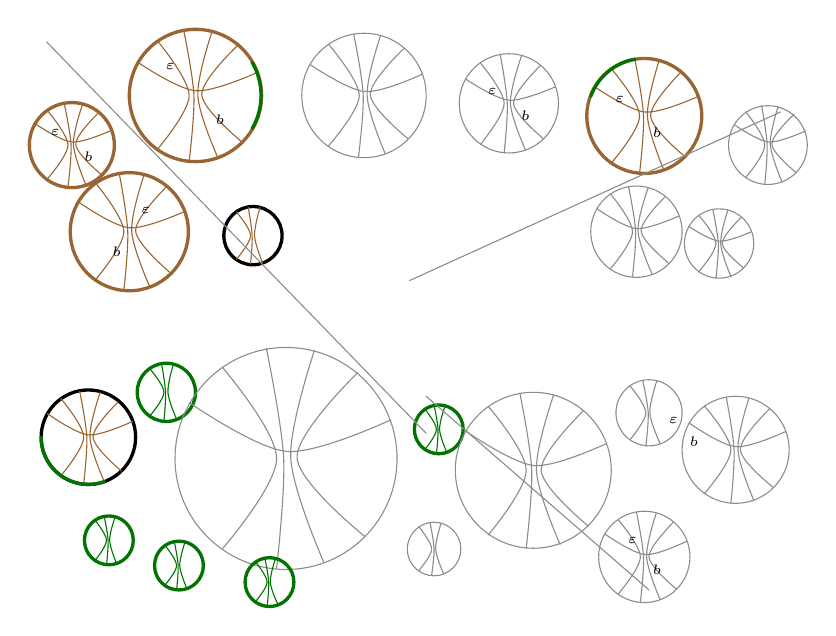
\begin{tikzpicture}[x=1mm,y=1mm,line cap=round,line join=round,font=\scriptsize]
\draw[Br,very thick] (5.8,-14.7) circle[radius=5.4];
\draw[Br] plot[smooth, tension=0.55] coordinates {(4.8,-9.3) (5.7,-14.7) (5.3,-20.1)};
\draw[Br] plot[smooth, tension=0.55] coordinates {(7.2,-9.4) (6,-14.6) (7.6,-19.8)};
\draw[Br] plot[smooth, tension=0.55] coordinates {(2.6,-10.2) (5.3,-14.7) (2.6,-19.1)};
\draw[Br] plot[smooth, tension=0.55] coordinates {(9.3,-10.5) (6.3,-14.6) (9.6,-18.5)};
\draw[Br] plot[smooth, tension=0.55] coordinates {(1,-11.9) (5.8,-14.3) (10.9,-12.8)};
\draw[Br,very thick] (21.5,-8.4) circle[radius=8.4];
\draw[Br] plot[smooth, tension=0.55] coordinates {(20,-0.1) (21.3,-8.4) (20.7,-16.7)};
\draw[Br] plot[smooth, tension=0.55] coordinates {(23.6,-0.3) (21.8,-8.4) (24.3,-16.2)};
\draw[Br] plot[smooth, tension=0.55] coordinates {(16.7,-1.5) (20.7,-8.4) (16.7,-15.2)};
\draw[Br] plot[smooth, tension=0.55] coordinates {(26.9,-2) (22.3,-8.3) (27.4,-14.3)};
\draw[Br] plot[smooth, tension=0.55] coordinates {(14.2,-4.2) (21.5,-7.8) (29.3,-5.5)};
\draw[pencil] (42.9,-8.4) circle[radius=7.9];
\draw[pencil] plot[smooth, tension=0.55] coordinates {(41.6,-0.6) (42.8,-8.4) (42.2,-16.2)};
\draw[pencil] plot[smooth, tension=0.55] coordinates {(45,-0.8) (43.3,-8.4) (45.6,-15.8)};
\draw[pencil] plot[smooth, tension=0.55] coordinates {(38.4,-1.9) (42.3,-8.4) (38.4,-14.8)};
\draw[pencil] plot[smooth, tension=0.55] coordinates {(48,-2.4) (43.7,-8.3) (48.5,-13.9)};
\draw[pencil] plot[smooth, tension=0.55] coordinates {(36.1,-4.5) (43,-7.9) (50.3,-5.7)};
\draw[pencil] (61.3,-9.4) circle[radius=6.3];
\draw[pencil] plot[smooth, tension=0.55] coordinates {(60.2,-3.2) (61.1,-9.4) (60.7,-15.7)};
\draw[pencil] plot[smooth, tension=0.55] coordinates {(62.9,-3.4) (61.5,-9.4) (63.4,-15.3)};
\draw[pencil] plot[smooth, tension=0.55] coordinates {(57.7,-4.3) (60.7,-9.4) (57.7,-14.6)};
\draw[pencil] plot[smooth, tension=0.55] coordinates {(65.3,-4.6) (61.9,-9.4) (65.7,-13.9)};
\draw[pencil] plot[smooth, tension=0.55] coordinates {(55.8,-6.3) (61.3,-9) (67.2,-7.3)};
\draw[Br,very thick] (78.5,-11) circle[radius=7.3];
\draw[Br] plot[smooth, tension=0.55] coordinates {(77.3,-3.8) (78.4,-11) (77.9,-18.3)};
\draw[Br] plot[smooth, tension=0.55] coordinates {(80.4,-3.9) (78.9,-11) (81,-17.9)};
\draw[Br] plot[smooth, tension=0.55] coordinates {(74.3,-5) (77.9,-11) (74.3,-17)};
\draw[Br] plot[smooth, tension=0.55] coordinates {(83.2,-5.4) (79.3,-11) (83.7,-16.2)};
\draw[Br] plot[smooth, tension=0.55] coordinates {(72.2,-7.3) (78.6,-10.5) (85.4,-8.5)};
\draw[pencil] (94.2,-14.7) circle[radius=5];
\draw[pencil] plot[smooth, tension=0.55] coordinates {(93.4,-9.7) (94.1,-14.7) (93.8,-19.7)};
\draw[pencil] plot[smooth, tension=0.55] coordinates {(95.5,-9.8) (94.5,-14.6) (96,-19.4)};
\draw[pencil] plot[smooth, tension=0.55] coordinates {(91.4,-10.5) (93.8,-14.7) (91.4,-18.8)};
\draw[pencil] plot[smooth, tension=0.55] coordinates {(97.5,-10.8) (94.7,-14.6) (97.8,-18.2)};
\draw[pencil] plot[smooth, tension=0.55] coordinates {(89.9,-12.1) (94.3,-14.3) (99,-12.9)};
\draw[Br,very thick] (13.1,-25.7) circle[radius=7.5];
\draw[Br] plot[smooth, tension=0.55] coordinates {(11.8,-18.2) (12.9,-25.7) (12.4,-33.2)};
\draw[Br] plot[smooth, tension=0.55] coordinates {(15,-18.4) (13.4,-25.6) (15.7,-32.7)};
\draw[Br] plot[smooth, tension=0.55] coordinates {(8.8,-19.5) (12.4,-25.7) (8.8,-31.8)};
\draw[Br] plot[smooth, tension=0.55] coordinates {(17.9,-19.9) (13.9,-25.6) (18.4,-31)};
\draw[Br] plot[smooth, tension=0.55] coordinates {(6.6,-21.9) (13.1,-25.2) (20.2,-23.1)};
\draw[very thick,very thick] (28.8,-26.2) circle[radius=3.7];
\draw[Br] plot[smooth, tension=0.55] coordinates {(28.2,-22.6) (28.7,-26.2) (28.5,-29.8)};
\draw[Br] plot[smooth, tension=0.55] coordinates {(29.7,-22.6) (29,-26.2) (30,-29.6)};
\draw[Br] plot[smooth, tension=0.55] coordinates {(26.7,-23.2) (28.5,-26.2) (26.7,-29.2)};
\draw[pencil] (77.5,-25.7) circle[radius=5.8];
\draw[pencil] plot[smooth, tension=0.55] coordinates {(76.5,-20) (77.4,-25.7) (77,-31.4)};
\draw[pencil] plot[smooth, tension=0.55] coordinates {(79,-20.1) (77.7,-25.6) (79.5,-31.1)};
\draw[pencil] plot[smooth, tension=0.55] coordinates {(74.2,-20.9) (77,-25.7) (74.2,-30.4)};
\draw[pencil] plot[smooth, tension=0.55] coordinates {(81.2,-21.2) (78.1,-25.6) (81.6,-29.7)};
\draw[pencil] plot[smooth, tension=0.55] coordinates {(72.5,-22.8) (77.5,-25.3) (82.9,-23.7)};
\draw[pencil] (88,-27.2) circle[radius=4.4];
\draw[pencil] plot[smooth, tension=0.55] coordinates {(87.2,-22.9) (87.9,-27.2) (87.6,-31.6)};
\draw[pencil] plot[smooth, tension=0.55] coordinates {(89.1,-23) (88.2,-27.2) (89.5,-31.4)};
\draw[pencil] plot[smooth, tension=0.55] coordinates {(85.4,-23.6) (87.6,-27.2) (85.4,-30.8)};
\draw[pencil] plot[smooth, tension=0.55] coordinates {(90.8,-23.9) (88.4,-27.2) (91.1,-30.3)};
\draw[pencil] plot[smooth, tension=0.55] coordinates {(84.1,-25) (88,-26.9) (92.1,-25.7)};
\draw[Dg,very thick] (17.8,-46.1) circle[radius=3.7];
\draw[Dg] plot[smooth, tension=0.55] coordinates {(17.2,-42.5) (17.7,-46.1) (17.5,-49.7)};
\draw[Dg] plot[smooth, tension=0.55] coordinates {(18.7,-42.5) (18,-46.1) (19.1,-49.5)};
\draw[Dg] plot[smooth, tension=0.55] coordinates {(15.7,-43.1) (17.5,-46.1) (15.7,-49.1)};
\draw[very thick,very thick] (7.9,-51.8) circle[radius=6];
\draw[Br] plot[smooth, tension=0.55] coordinates {(6.8,-46) (7.7,-51.8) (7.3,-57.8)};
\draw[Br] plot[smooth, tension=0.55] coordinates {(9.4,-46.1) (8.1,-51.8) (9.9,-57.4)};
\draw[Br] plot[smooth, tension=0.55] coordinates {(4.4,-46.9) (7.3,-51.8) (4.4,-56.7)};
\draw[Br] plot[smooth, tension=0.55] coordinates {(11.7,-47.3) (8.5,-51.8) (12.1,-56.1)};
\draw[Br] plot[smooth, tension=0.55] coordinates {(2.7,-48.8) (7.9,-51.5) (13.5,-49.8)};
\draw[pencil] (33,-54.5) circle[radius=14.1];
\draw[pencil] plot[smooth, tension=0.55] coordinates {(30.5,-40.5) (32.7,-54.5) (31.8,-68.5)};
\draw[pencil] plot[smooth, tension=0.55] coordinates {(36.6,-40.8) (33.6,-54.4) (37.8,-67.7)};
\draw[pencil] plot[smooth, tension=0.55] coordinates {(24.9,-42.9) (31.8,-54.5) (24.9,-66)};
\draw[pencil] plot[smooth, tension=0.55] coordinates {(42.1,-43.6) (34.4,-54.4) (43,-64.4)};
\draw[pencil] plot[smooth, tension=0.55] coordinates {(20.7,-47.4) (33.1,-53.6) (46.3,-49.6)};
\draw[Dg,very thick] (52.4,-50.8) circle[radius=3.1];
\draw[Dg] plot[smooth, tension=0.55] coordinates {(51.8,-47.7) (52.3,-50.8) (52.1,-53.9)};
\draw[Dg] plot[smooth, tension=0.55] coordinates {(53.2,-47.8) (52.5,-50.8) (53.4,-53.7)};
\draw[Dg] plot[smooth, tension=0.55] coordinates {(50.6,-48.2) (52.1,-50.8) (50.6,-53.4)};
\draw[pencil] (64.4,-56) circle[radius=9.9];
\draw[pencil] plot[smooth, tension=0.55] coordinates {(62.7,-46.2) (64.2,-56) (63.5,-65.9)};
\draw[pencil] plot[smooth, tension=0.55] coordinates {(67,-46.4) (64.8,-56) (67.8,-65.4)};
\draw[pencil] plot[smooth, tension=0.55] coordinates {(58.7,-47.9) (63.5,-56) (58.7,-64.2)};
\draw[pencil] plot[smooth, tension=0.55] coordinates {(70.8,-48.4) (65.4,-56) (71.4,-63.1)};
\draw[pencil] plot[smooth, tension=0.55] coordinates {(55.8,-51) (64.5,-55.4) (73.7,-52.6)};
\draw[pencil] (79.1,-48.7) circle[radius=4.2];
\draw[pencil] plot[smooth, tension=0.55] coordinates {(78.3,-44.6) (79,-48.7) (78.7,-52.9)};
\draw[pencil] plot[smooth, tension=0.55] coordinates {(80.1,-44.6) (79.2,-48.7) (80.5,-52.6)};
\draw[pencil] plot[smooth, tension=0.55] coordinates {(76.7,-45.3) (78.7,-48.7) (76.7,-52.1)};
\draw[pencil] (90.1,-53.4) circle[radius=6.8];
\draw[pencil] plot[smooth, tension=0.55] coordinates {(88.9,-46.7) (89.9,-53.4) (89.5,-60.2)};
\draw[pencil] plot[smooth, tension=0.55] coordinates {(91.8,-46.8) (90.4,-53.4) (92.4,-59.8)};
\draw[pencil] plot[smooth, tension=0.55] coordinates {(86.1,-47.8) (89.5,-53.4) (86.1,-59)};
\draw[pencil] plot[smooth, tension=0.55] coordinates {(94.4,-48.2) (90.7,-53.4) (94.9,-58.2)};
\draw[pencil] plot[smooth, tension=0.55] coordinates {(84.2,-50) (90.1,-53) (96.4,-51.1)};
\draw[Dg,very thick] (10.5,-64.9) circle[radius=3.1];
\draw[Dg] plot[smooth, tension=0.55] coordinates {(9.9,-61.8) (10.4,-64.9) (10.2,-68.1)};
\draw[Dg] plot[smooth, tension=0.55] coordinates {(11.3,-61.9) (10.6,-64.9) (11.5,-67.9)};
\draw[Dg] plot[smooth, tension=0.55] coordinates {(8.7,-62.3) (10.2,-64.9) (8.7,-67.5)};
\draw[Dg,very thick] (19.4,-68.1) circle[radius=3.1];
\draw[Dg] plot[smooth, tension=0.55] coordinates {(18.8,-65) (19.3,-68.1) (19.1,-71.2)};
\draw[Dg] plot[smooth, tension=0.55] coordinates {(20.2,-65) (19.5,-68.1) (20.4,-71)};
\draw[Dg] plot[smooth, tension=0.55] coordinates {(17.6,-65.5) (19.1,-68.1) (17.6,-70.6)};
\draw[Dg,very thick] (30.9,-70.2) circle[radius=3.1];
\draw[Dg] plot[smooth, tension=0.55] coordinates {(30.3,-67.1) (30.8,-70.2) (30.6,-73.3)};
\draw[Dg] plot[smooth, tension=0.55] coordinates {(31.7,-67.1) (31,-70.2) (32,-73.1)};
\draw[Dg] plot[smooth, tension=0.55] coordinates {(29.1,-67.6) (30.6,-70.2) (29.1,-72.7)};
\draw[pencil] (51.8,-66) circle[radius=3.4];
\draw[pencil] plot[smooth, tension=0.55] coordinates {(51.3,-62.7) (51.8,-66) (51.5,-69.3)};
\draw[pencil] plot[smooth, tension=0.55] coordinates {(52.7,-62.7) (52,-66) (53,-69.1)};
\draw[pencil] plot[smooth, tension=0.55] coordinates {(49.9,-63.2) (51.5,-66) (49.9,-68.7)};
\draw[pencil] (78.5,-67) circle[radius=5.8];
\draw[pencil] plot[smooth, tension=0.55] coordinates {(77.5,-61.3) (78.4,-67) (78,-72.8)};
\draw[pencil] plot[smooth, tension=0.55] coordinates {(80,-61.5) (78.8,-67) (80.5,-72.4)};
\draw[pencil] plot[smooth, tension=0.55] coordinates {(75.2,-62.3) (78,-67) (75.2,-71.7)};
\draw[pencil] plot[smooth, tension=0.55] coordinates {(82.2,-62.6) (79.1,-67) (82.6,-71.1)};
\draw[pencil] plot[smooth, tension=0.55] coordinates {(73.5,-64.1) (78.6,-66.7) (83.9,-65)};
\draw[Dg,very thick] (28.7,-12.6) arc[start angle=-30, end angle=30, x radius=8.4, y radius=8.4];
\draw[Dg,very thick] (77.3,-3.8) arc[start angle=100, end angle=160, x radius=7.3, y radius=7.3];
\draw[Dg,very thick] (1.9,-51.8) arc[start angle=180, end angle=290, x radius=6, y radius=6];
\node[inner sep=1pt] at (3.7,-13.1) {\tiny $\varepsilon$};
\node[inner sep=1pt] at (7.9,-16.2) {\tiny $b$};
\node[inner sep=1pt] at (18.3,-4.7) {\tiny $\varepsilon$};
\node[inner sep=1pt] at (24.6,-11.5) {\tiny $b$};
\node[inner sep=1pt] at (15.2,-23) {\tiny $\varepsilon$};
\node[inner sep=1pt] at (11.5,-28.3) {\tiny $b$};
\node[inner sep=1pt] at (59.2,-7.9) {\tiny $\varepsilon$};
\node[inner sep=1pt] at (63.4,-11) {\tiny $b$};
\node[inner sep=1pt] at (75.4,-8.9) {\tiny $\varepsilon$};
\node[inner sep=1pt] at (80.1,-13.1) {\tiny $b$};
\node[inner sep=1pt] at (82.2,-49.7) {\tiny $\varepsilon$};
\node[inner sep=1pt] at (84.8,-52.4) {\tiny $b$};
\node[inner sep=1pt] at (77,-64.9) {\tiny $\varepsilon$};
\node[inner sep=1pt] at (80.1,-68.6) {\tiny $b$};
\draw[pencil] (2.6,-1.6) -- (50.8,-51.3);
\draw[pencil] (48.7,-31.9) -- (95.8,-10.5);
\draw[pencil] (50.8,-46.6) -- (79.1,-71.2);
\end{tikzpicture}
\end{document}
